%% Additional packages

\documentclass[a4paper, 12pt]{article}
\usepackage{fontspec}
\usepackage{graphicx}
\usepackage{hyperref}
\usepackage[margin=1.5cm]{geometry}
\usepackage{amsmath}
\usepackage[polish]{babel}

%% Title

\title{\textbf{Symulacja ruchu ludzi w centrum handlowym}}
\author{Paweł Kłeczek \and Kajetan Rzepecki}
\date{2012-11-05}


%% Text starts here:
\begin{document}

    \vspace{\fill}
    \maketitle
    \vspace{\fill}
    \thispagestyle{empty}

\newpage
    \setcounter{page}{1}
    \setcounter{tocdepth}{3}
    \tableofcontents

\newpage
    \section{Wprowadzenie}
    \label{sec:intro}

    \noindent
    Celem wykonywanego projektu jest stworzenie modelu oraz symulacja ruchu ludzi w centrum handlowym w oparciu o model \hyperref[refs:social-distances-1]{Social Distances}.

    % TODO Wincyj by się przydało tego wprowadzenia...
    % TODO Nie mam żadnego pomysłu poza nawiązaniem do innych, podobnych symulacji.

    \begin{figure}[h!]
        \centering
        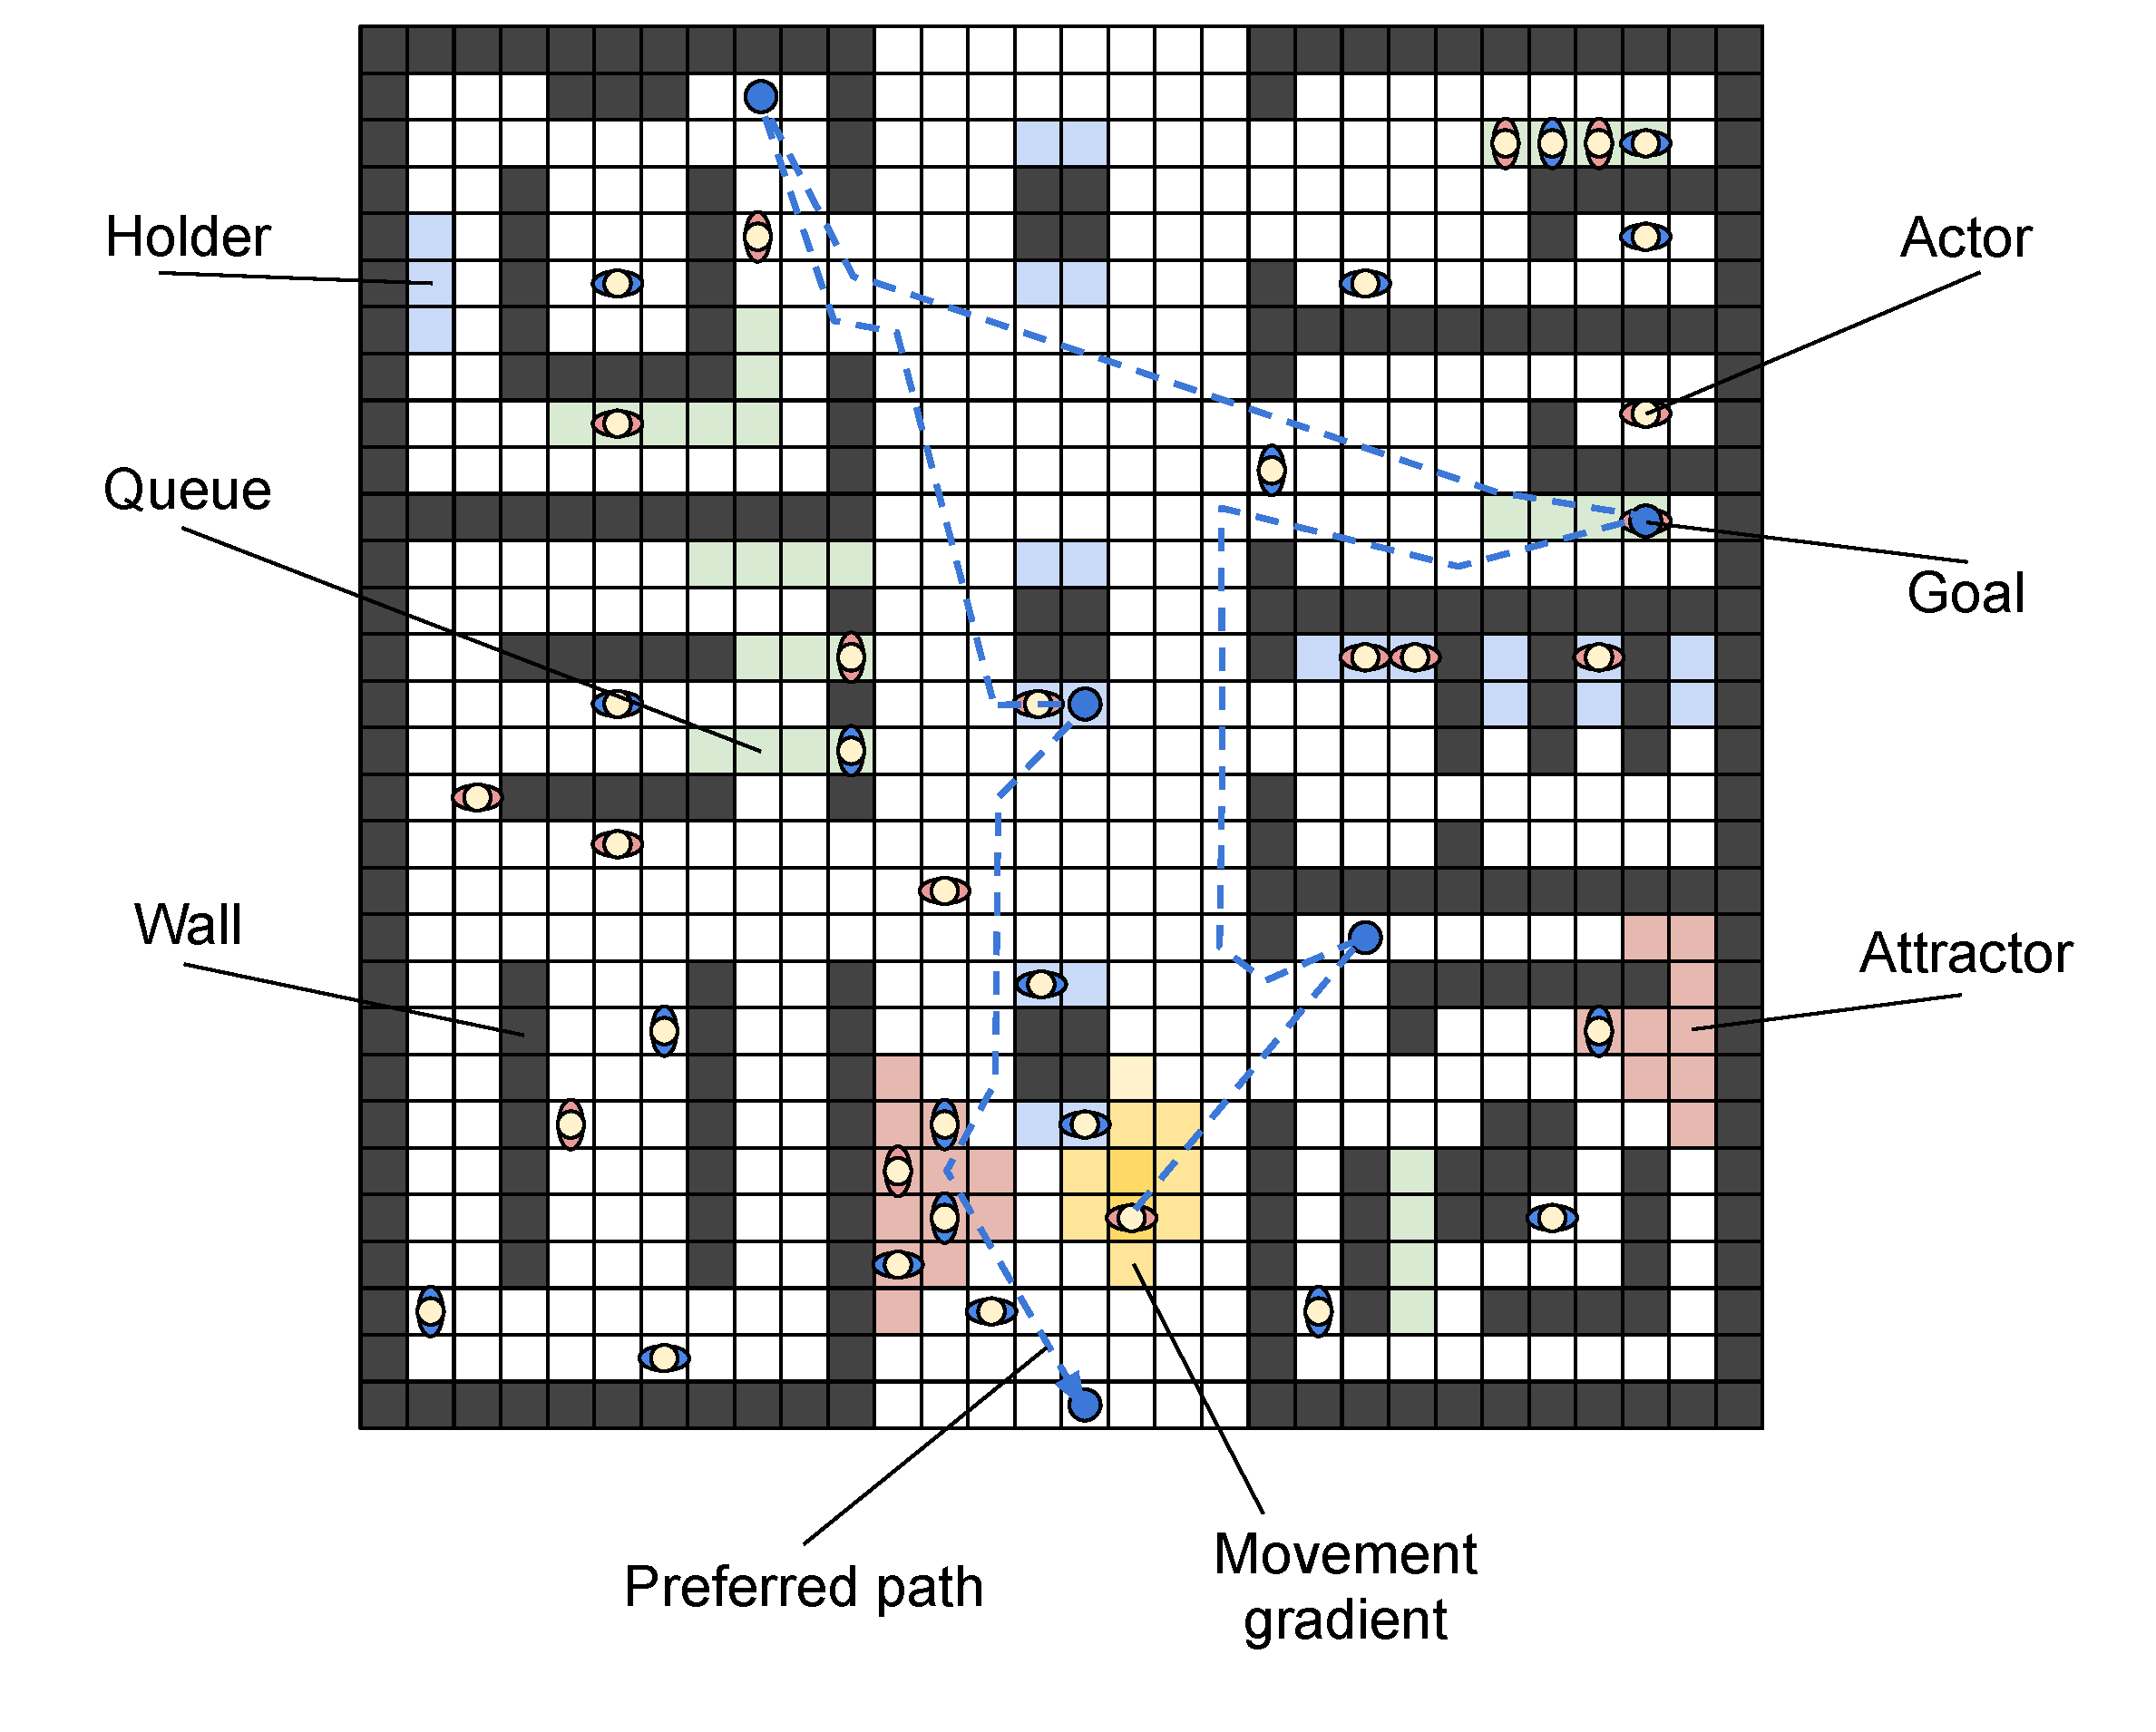
\includegraphics[scale=0.3]{./img/Overview.pdf}
        \caption{Przykładowa dekompozycja problemu.}
        \label{fig:overview}
    \end{figure}

    % TODO Opis fig:overview

\newpage
    \section{Centrum handlowe}
    \label{sec:mall}

    % TODO Opis reprezentacji centrum handlowego - atraktory, kolejki, schody, piętra itd.
    % TODO Uprzednio dobrze by było uściślić to, co ustaliliśmy na ten temat.

\newpage
    \section{Model ruchu ludzi}
    \label{sec:model}

    \noindent
    W zastosowanym algorytmie można wyszczególnieć dwie główne, wzajemnie od siebie zależne fazy - fazę \hyperref[sec:tactical]{taktyczną} oraz fazę \hyperref[sec:operational]{operacyjną}, których interakcję przestawiono na poniższym, uproszczonym diagramie.

    \begin{figure}[h!]
        \centering
        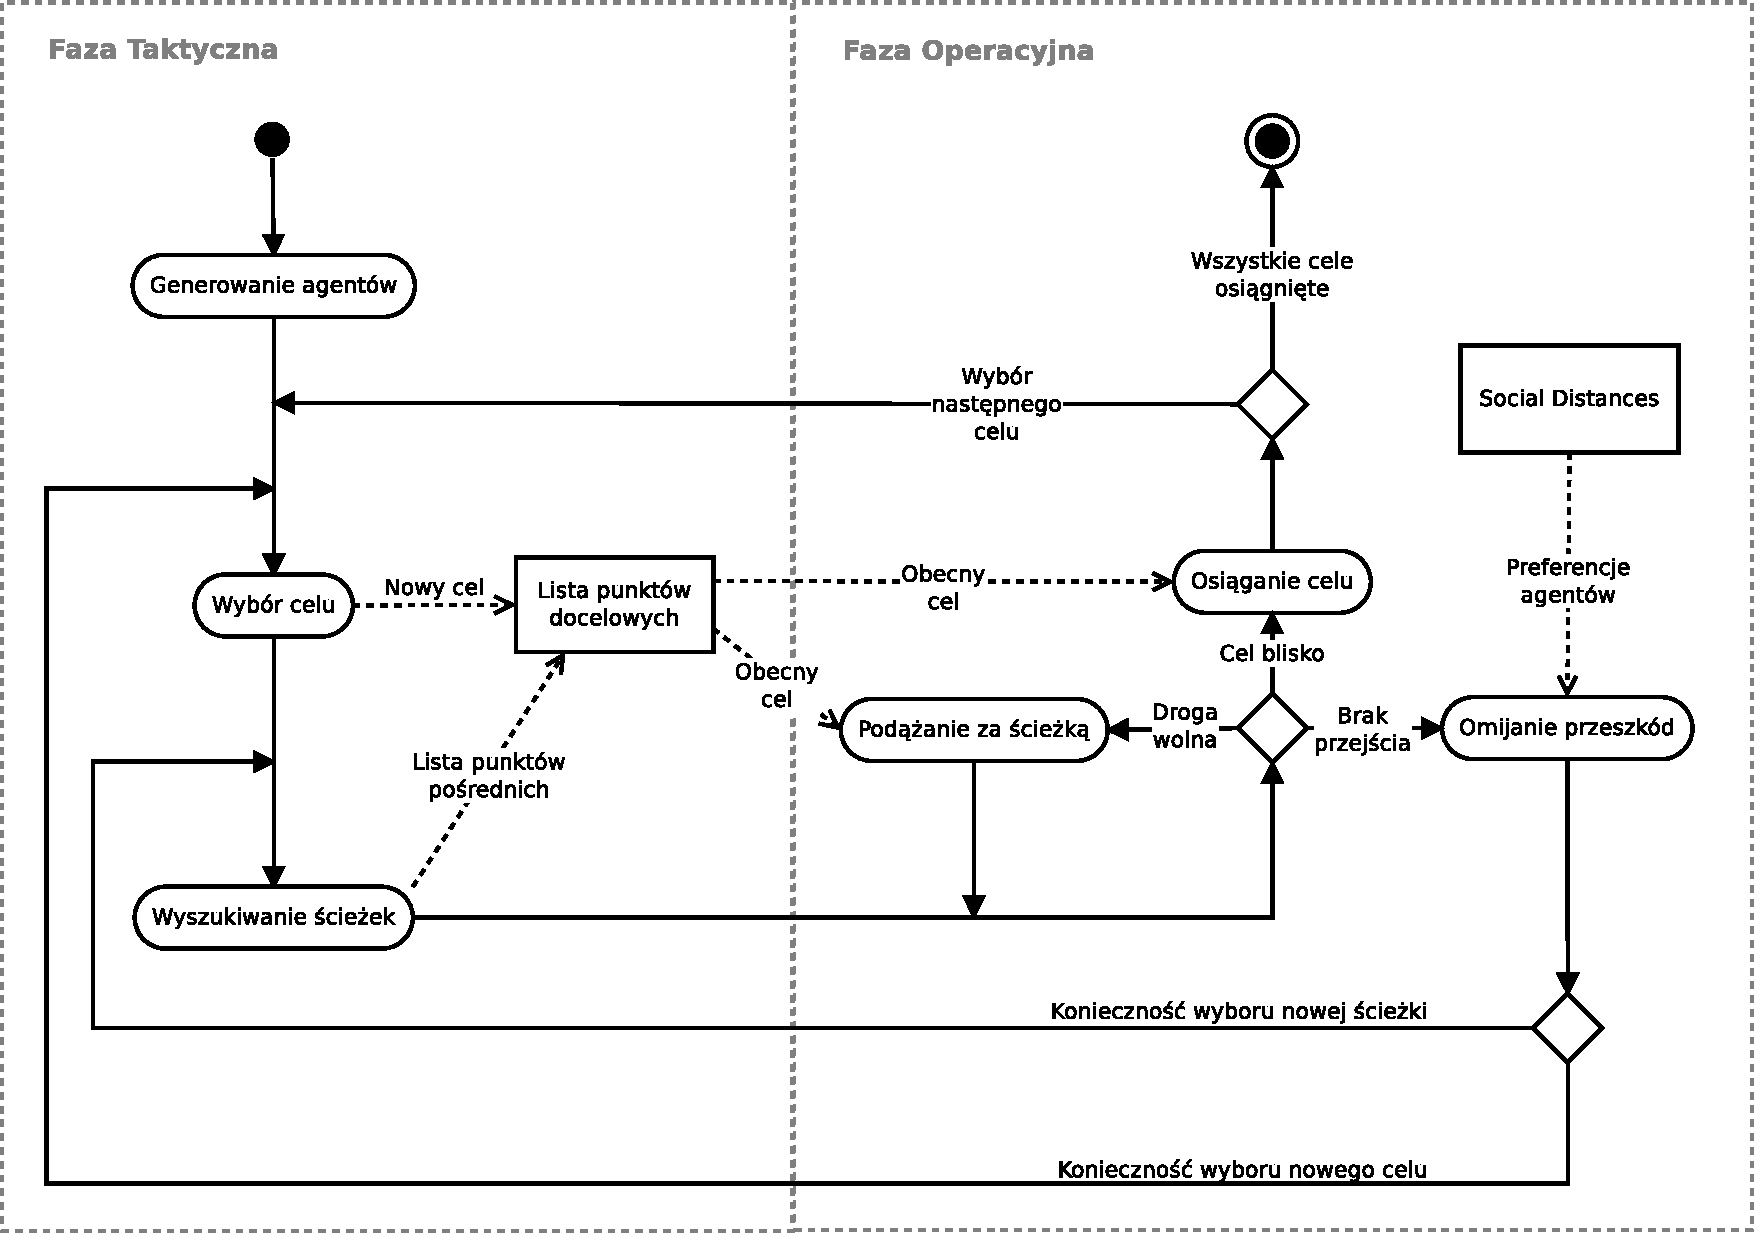
\includegraphics[scale=0.7]{./img/ActorActivity.pdf}
        \caption{Diagram aktywności aktorów.}
        \label{fig:actor-activity}
    \end{figure}

    % TODO Więcej szczegółów na temat generowania aktora i zestawu jego parametrów.
    % TODO Więcej szczegółów na temat algorytmu wybierania miejsc docelonych.
    % TODO Link do opisu stref specjalnych centrum handlowego.

    Algorytm rozpoczyna pracę od wygenerowania aktora na podstawie wcześniej zdefiniowanych schematów.
Dla każdego aktora wybierana jest wstępna lista miejsc docelowych, które zostaną przez niego odwiedzone w cziasie działania symulacji, oraz obliczana jest optymalna ścieżka wiodące do pierwszego wybranego w poprzednim kroku miejsca docelowego. Algorytm następnie modyfikuje ścieżkę w oparciu o mapę rozkładu stref specjalnych centrum handlowego by lepiej modelować faktyczne zamiary danego aktora.

    Po wygenerowaniu niezbędnych danych taktycznych dla każdego aktora algorytm przechodzi do fazy operacyjnej, która odpowiada za właściwy ruch aktorów. Faza ta zachodzi w lokalnym otoczeniu każdego agenta i odpowiada za zachowania takie jak omijanie przeszkód, grupowanie się, podążanie za ścieżką i inne akcje związane ze specjalnymi strefami centrum handlowego.
Algorytm na podstawie bezpośredniego otoczenia aktora oraz metadanych dotyczących obecnego celu jego podróży podejmuje decyzje o możliwości wykonania ruchu, lub w przypadku skrajnym o modyfikacji wybranej ścieżki prowadzącej do celu, czy nawet modyfikacji aktualnego celu podróży.
W przypadku osiągnięcia miejsca docelowego algorytm przechodzi do rozpatrywania następnego miejsca docelowego, lub w tryb ``błądzenia'', gdy osiągnięto ostatni cel.

\newpage
        \subsection{Faza taktyczna}
        \label{sec:tactical}

        \begin{figure}[h!]
            \centering
            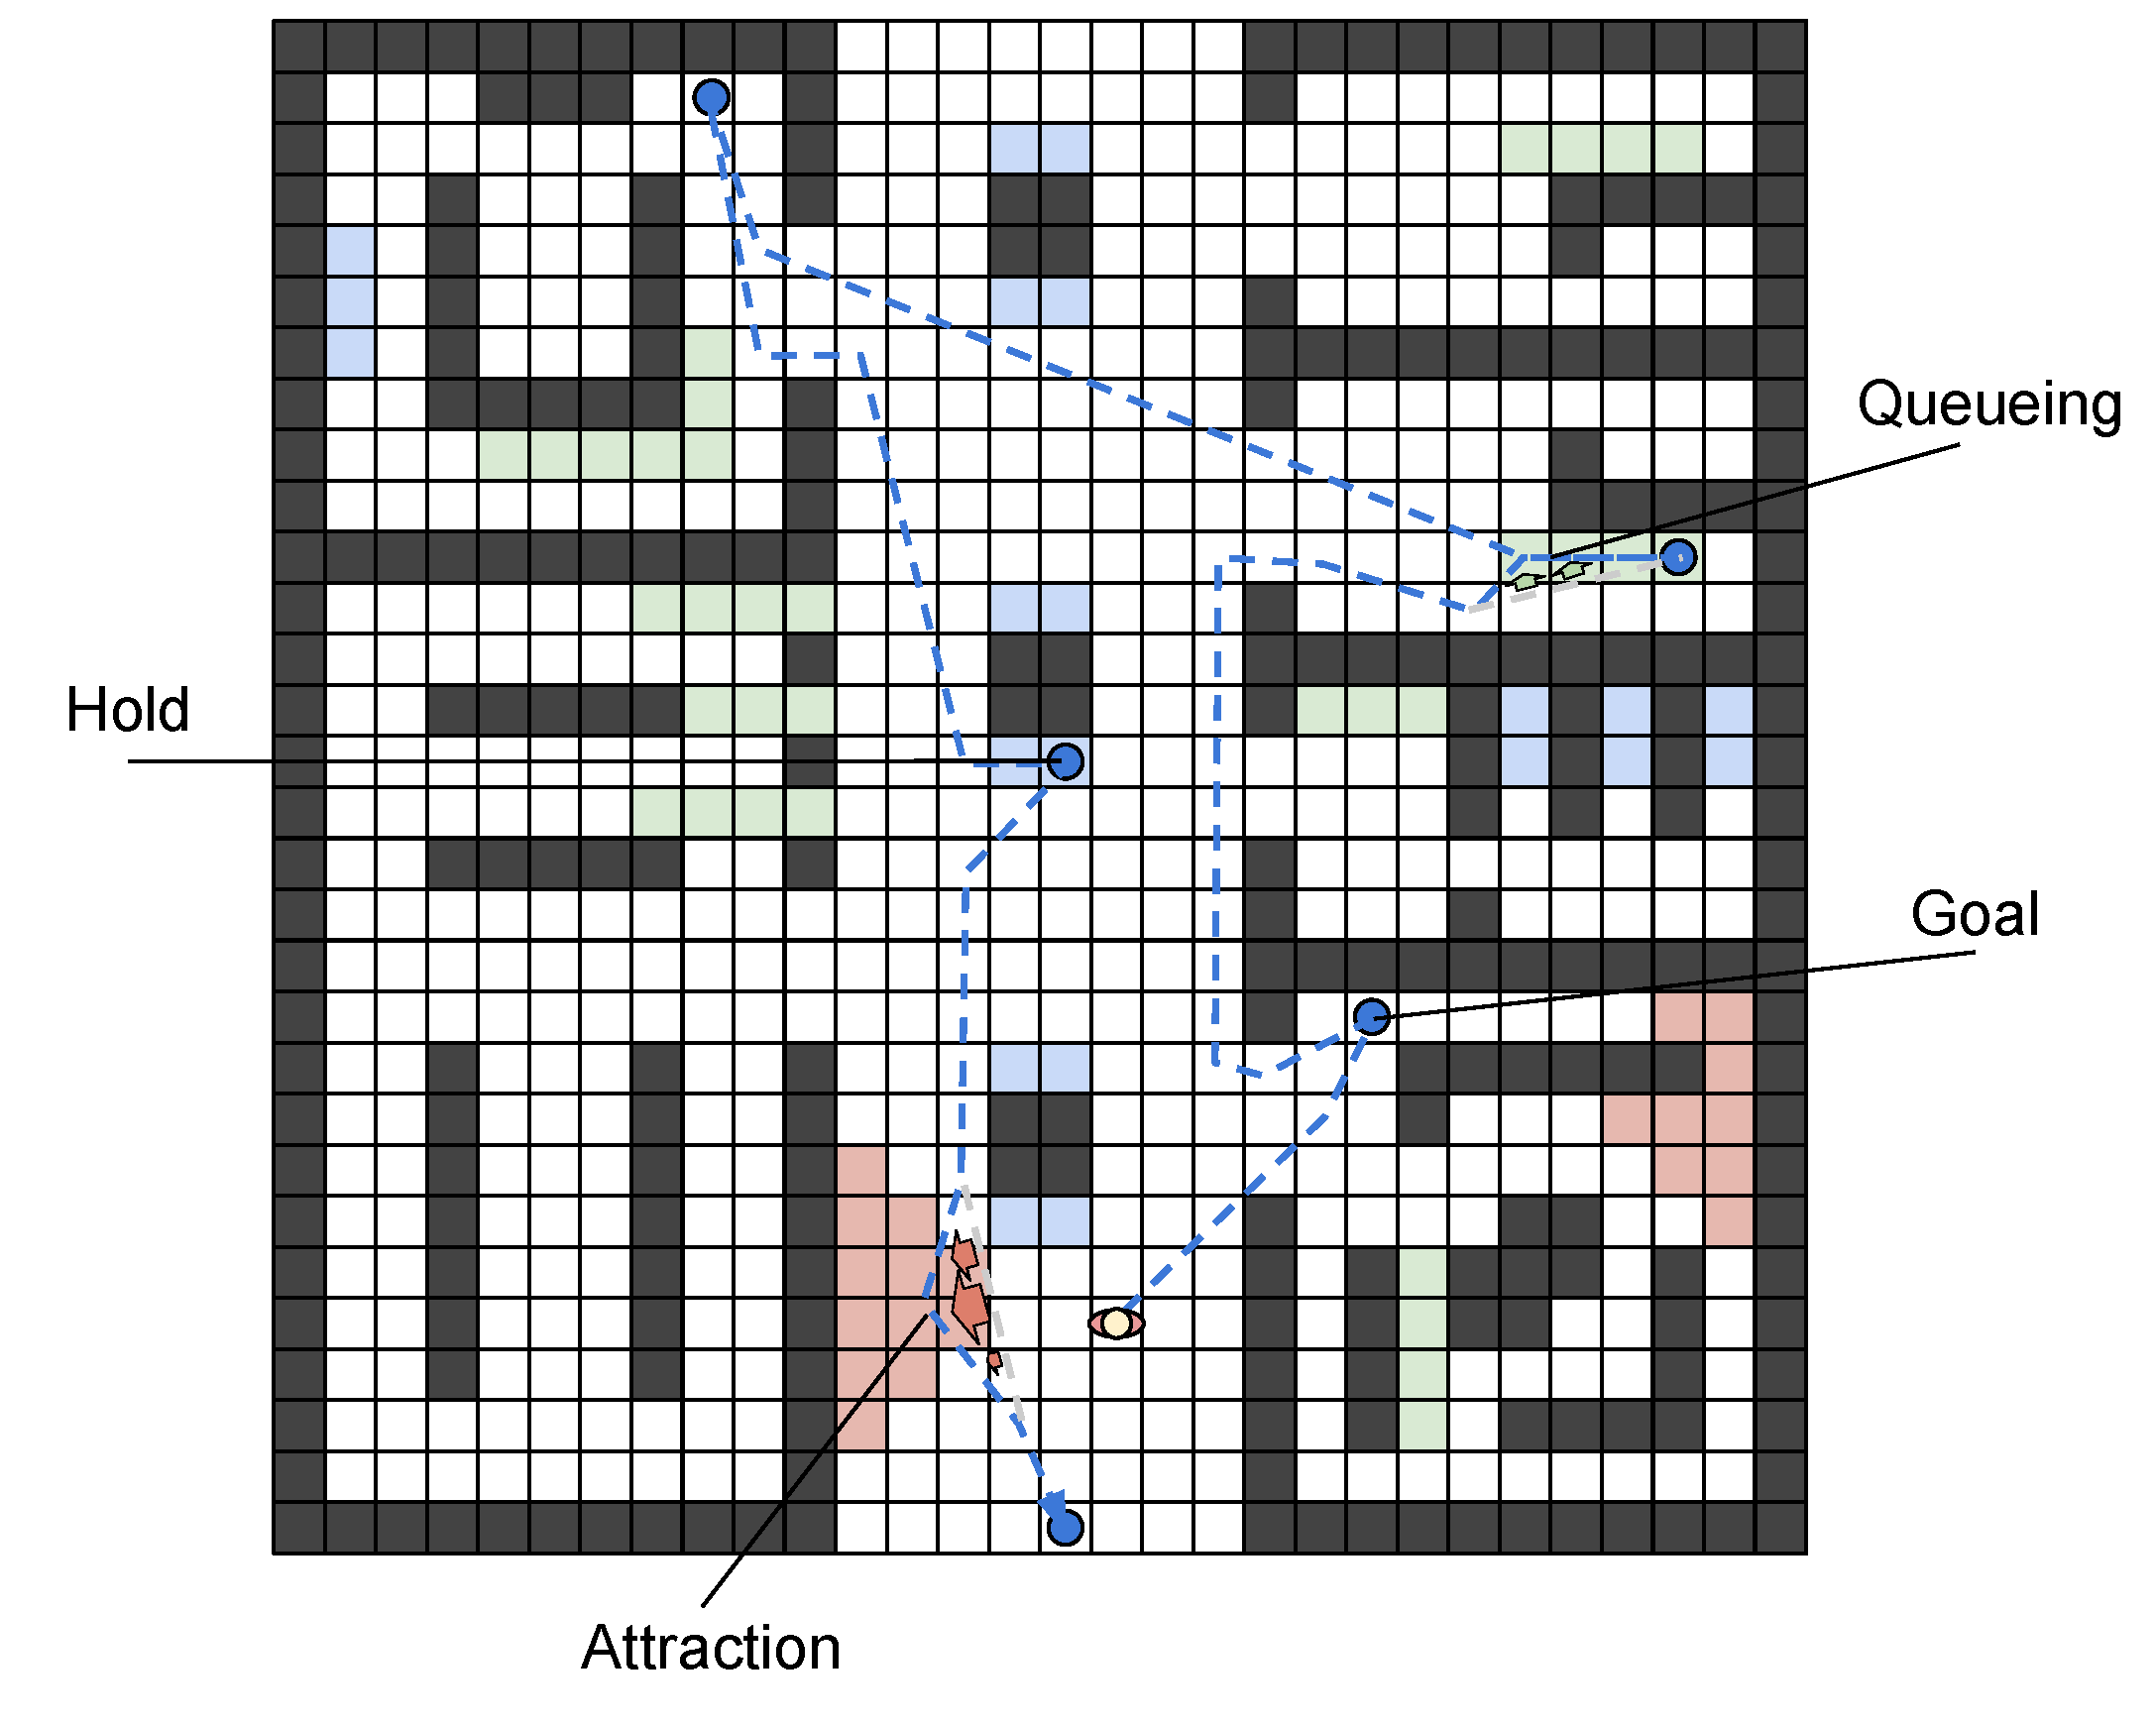
\includegraphics[scale=0.3]{./img/Tactical.pdf}
            \caption{Zakres operacji taktycznej części modelu ruchu.}
            \label{fig:tactical}
        \end{figure}

        % TODO Linki do opisu atraktorów, kolejek itd.

        \noindent
        Faza taktyczna zachodzi globalnie dla każdego aktora bez uwzględnienia jego lokalnego otoczenia, innych aktorów, czy technicznych właściwości centrum handlowego - nie jest istotnym, czy dany korytarz został zablokowany przez grupę ludzi i nie umożliwia przejścia. Faza ta modeluje abstrakcyjne zamiary aktora i jej celem jest przede wszystkim wybór listy miejsc docelowych oraz wyznaczenie dróg do nich prowadzących, co zostało osiągnięte dzięki algorytmowi znajdowania ścieżek oraz mapie rozkładu stref specjalnych centrum handlowego. Pod uwagę brane są atraktory, kolejki i schody, które algorytm stara się osiągnąć modyfikując wcześniej wyznaczoną, optymalną ścieżkę prowadzącą do aktualnego celu podróży.

        \subsection{Faza operacyjna}
        \label{sec:operational}

        \begin{figure}[h!]
            \centering
            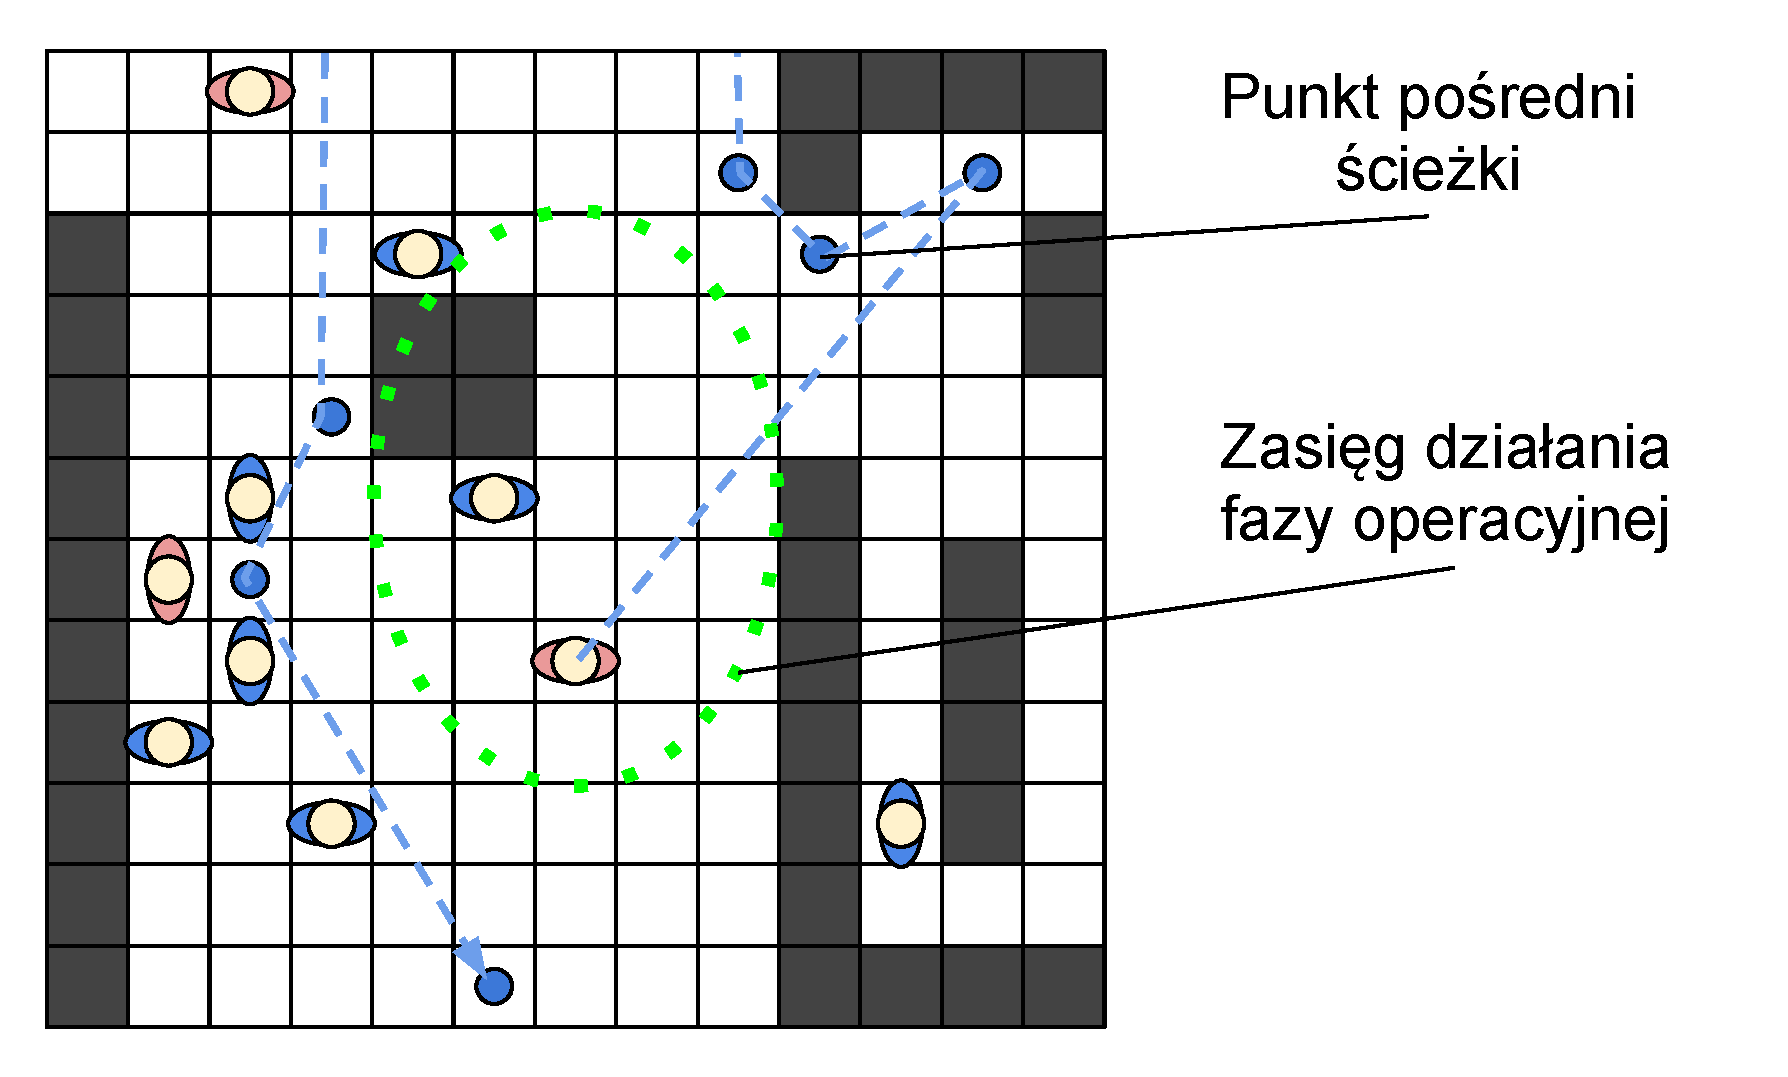
\includegraphics[scale=0.3]{./img/Operative.pdf}
            \caption{Zakres działania operacyjnej części modelu ruchu.}
            \label{fig:operational}
        \end{figure}

        % TODO Potrzeba większego opisu, który bardziej zagłębia się w wybrany algorytm operacyjny.

        \noindent
        Faza operacyjna zachodzi w lokalnym otoczeniu każdego aktora, a jej celem jest wykonanie właściwego ruchu aktora. Faza ta jest odpowiedzialna za unikanie kolizji i omijanie przeszkód. Pod uwagę brani są inni aktorzy oraz metadane dotyczące drogi prowadzącej do aktualnego celu podróży wygenerowane w taktyczniej fazie działania algorytmu.

\newpage
    \section{Implementacja}
    \label{sec:implementation}

        \subsection{Reprezentacja centrum handlowego}
        \label{sec:mall-impl}

        \begin{figure}[h!]
            \centering
            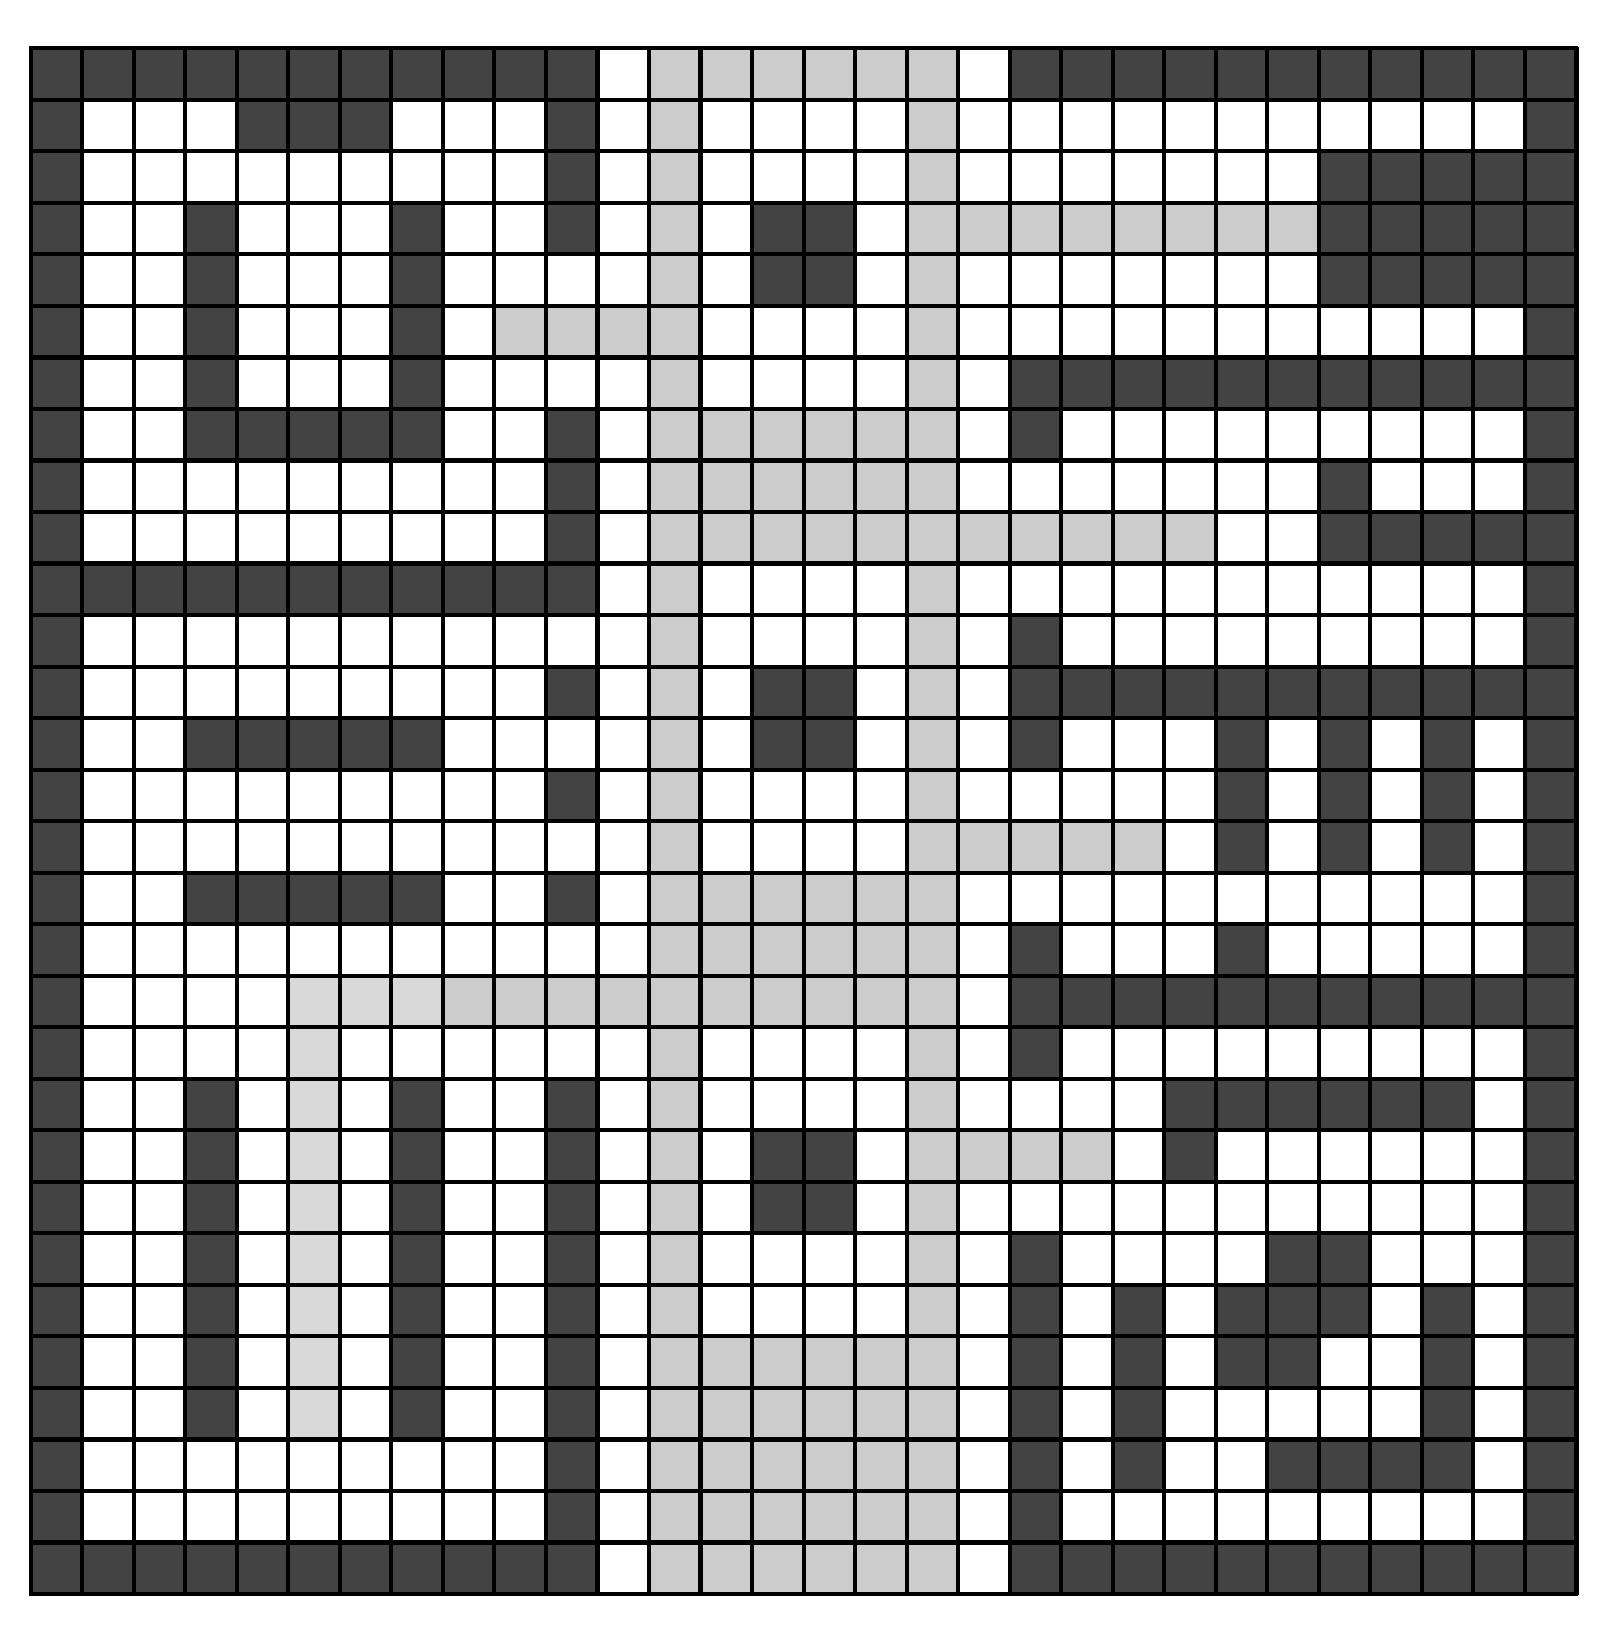
\includegraphics[scale=0.2]{./img/MallLayout.pdf}
            \caption{Przykładowy rozkład pomieszczeń małego centrum handlowego.}
            \label{fig:mall-layout}
        \end{figure}

        \begin{figure}[h!]
            \centering
            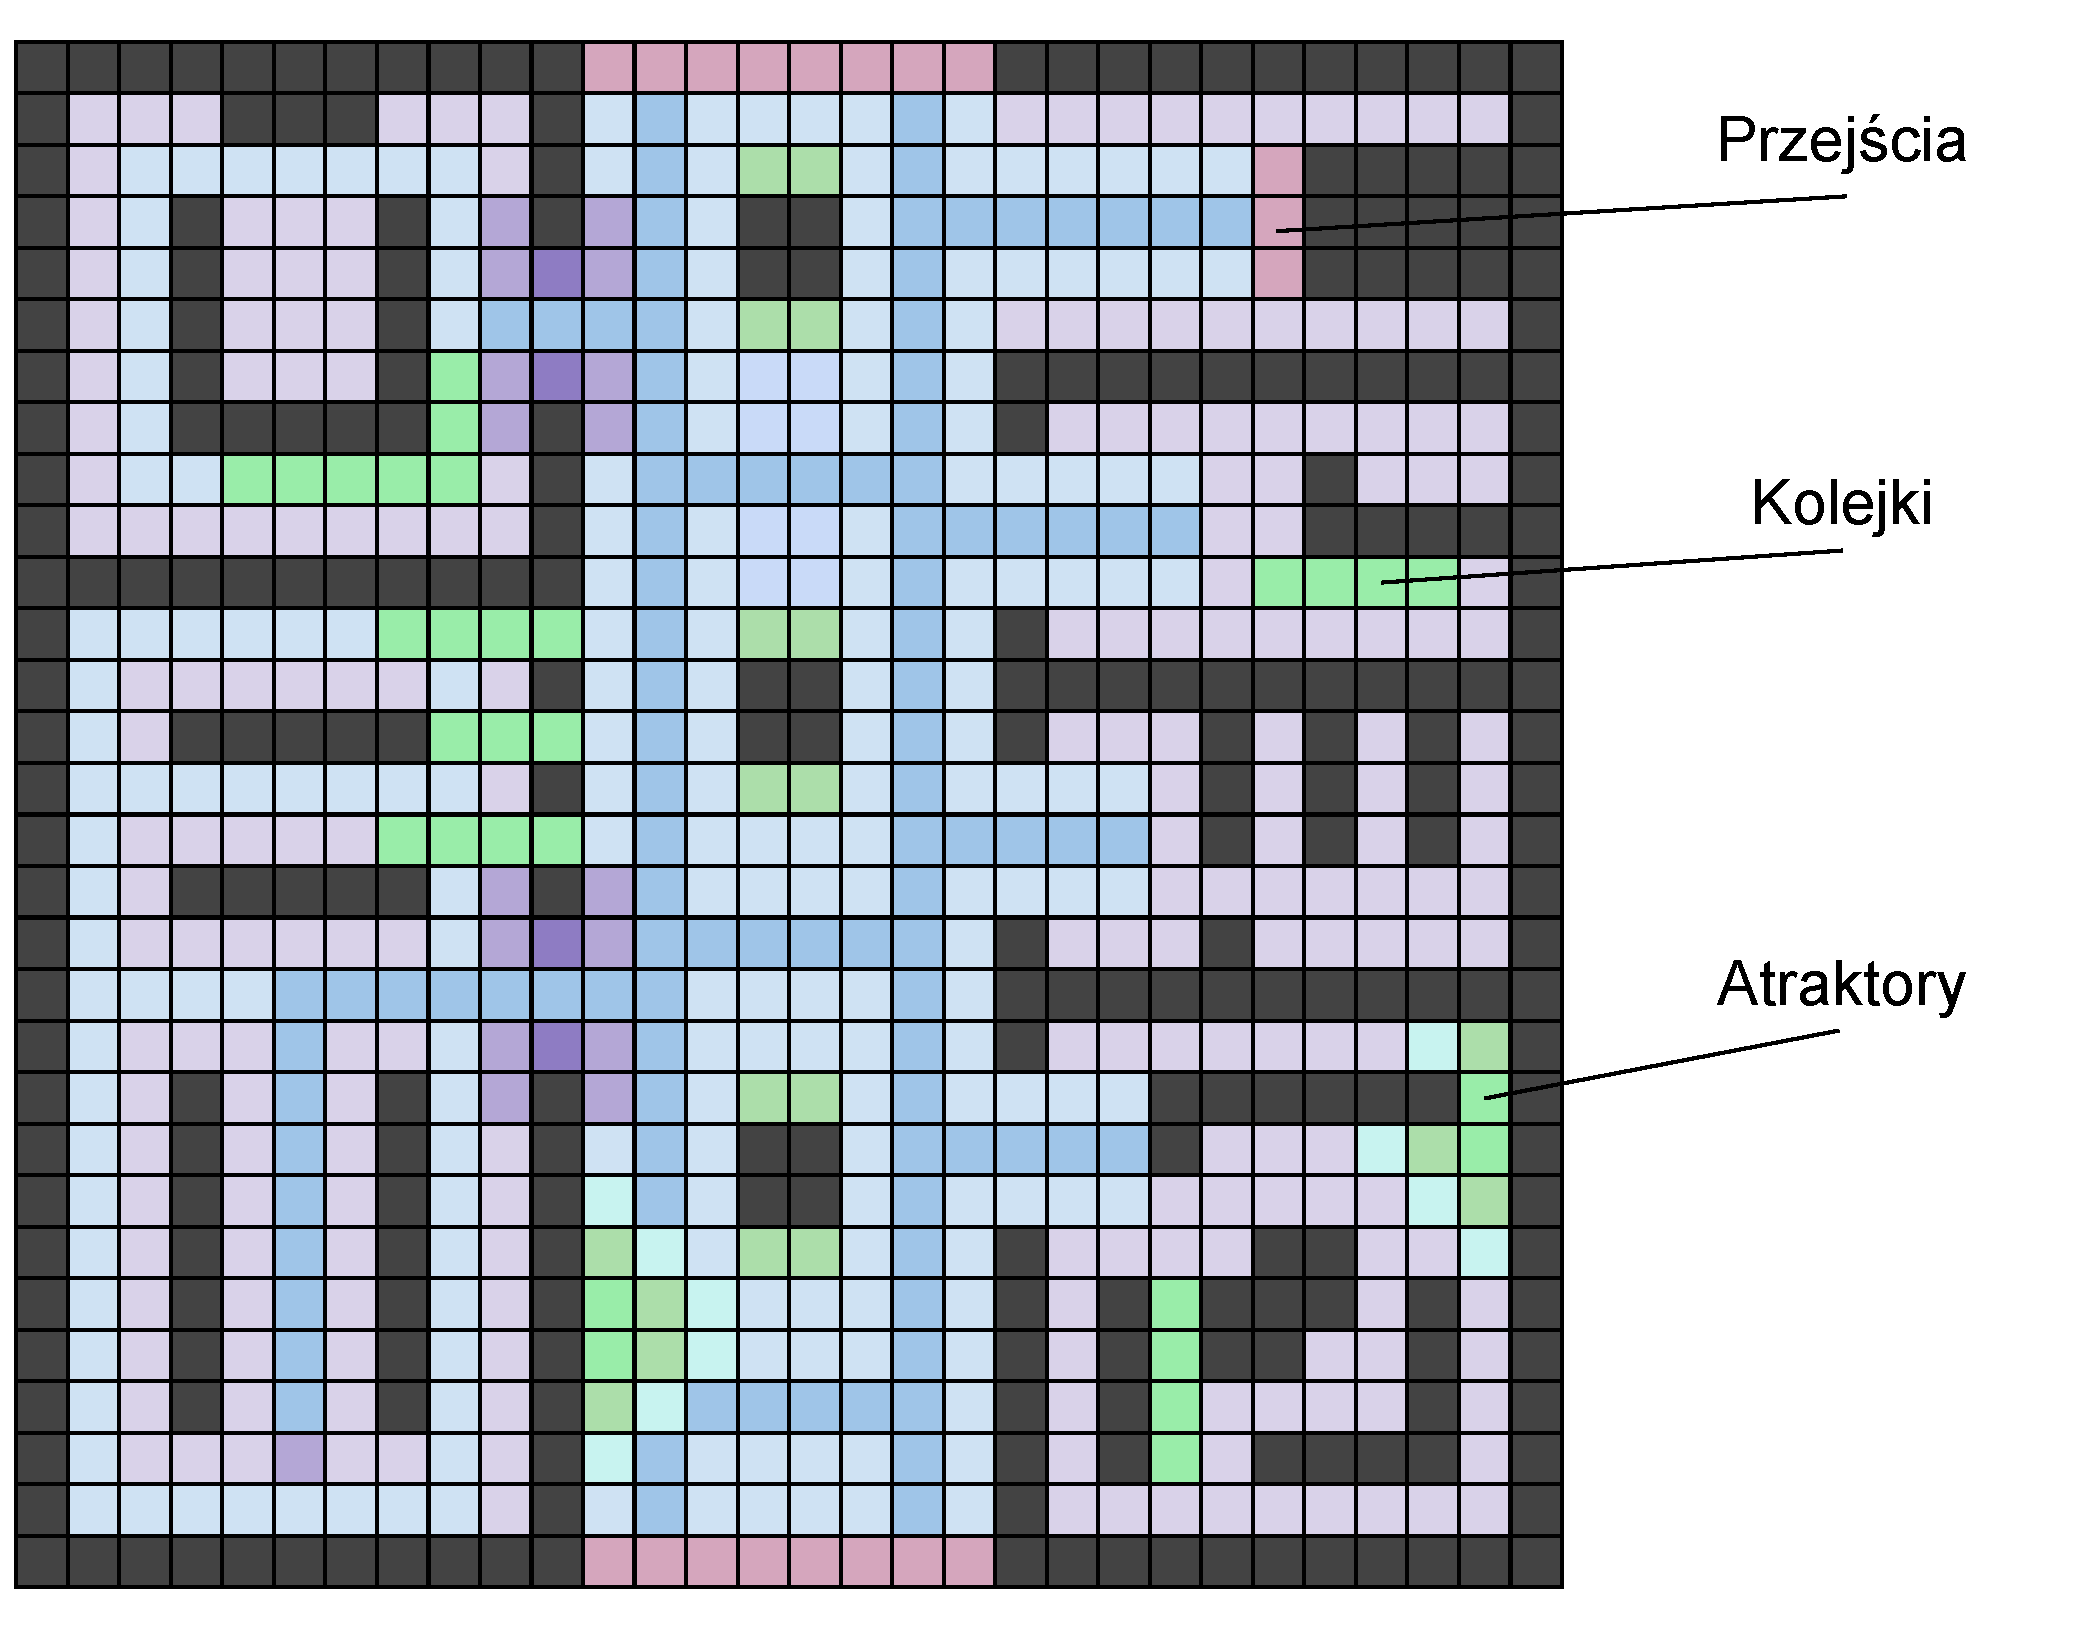
\includegraphics[scale=0.2]{./img/MallFeatures.pdf}
            \caption{Przykładowy rozkład stref specjalnych małego centrum handlowego.}
            \label{fig:mall-features}
        \end{figure}


     % TODO Trzeba zweryfikować i opisać technikalia implementacji...
     % TODO Ofkors po uprzednim zaimplementowaniu całości ;)
\newpage
    \section{Referencje}
    \label{sec:refs}

    \begin{itemize}
        % TODO Trzeba wybrać jedną do dwóch publikacji, które zgrabnie opisują model Social Distances.
        \begin{item} \label{refs:social-distances-1} Social Distances \end{item}
        \item \ldots %% TODO Moar
    \end{itemize}
\end{document}
